\begin{frame}
\frametitle{三栏图文混排}
\framesubtitle{图片 · 表格 · 绘图}

\begin{columns}[T]
\column{0.32\textwidth}
\centering
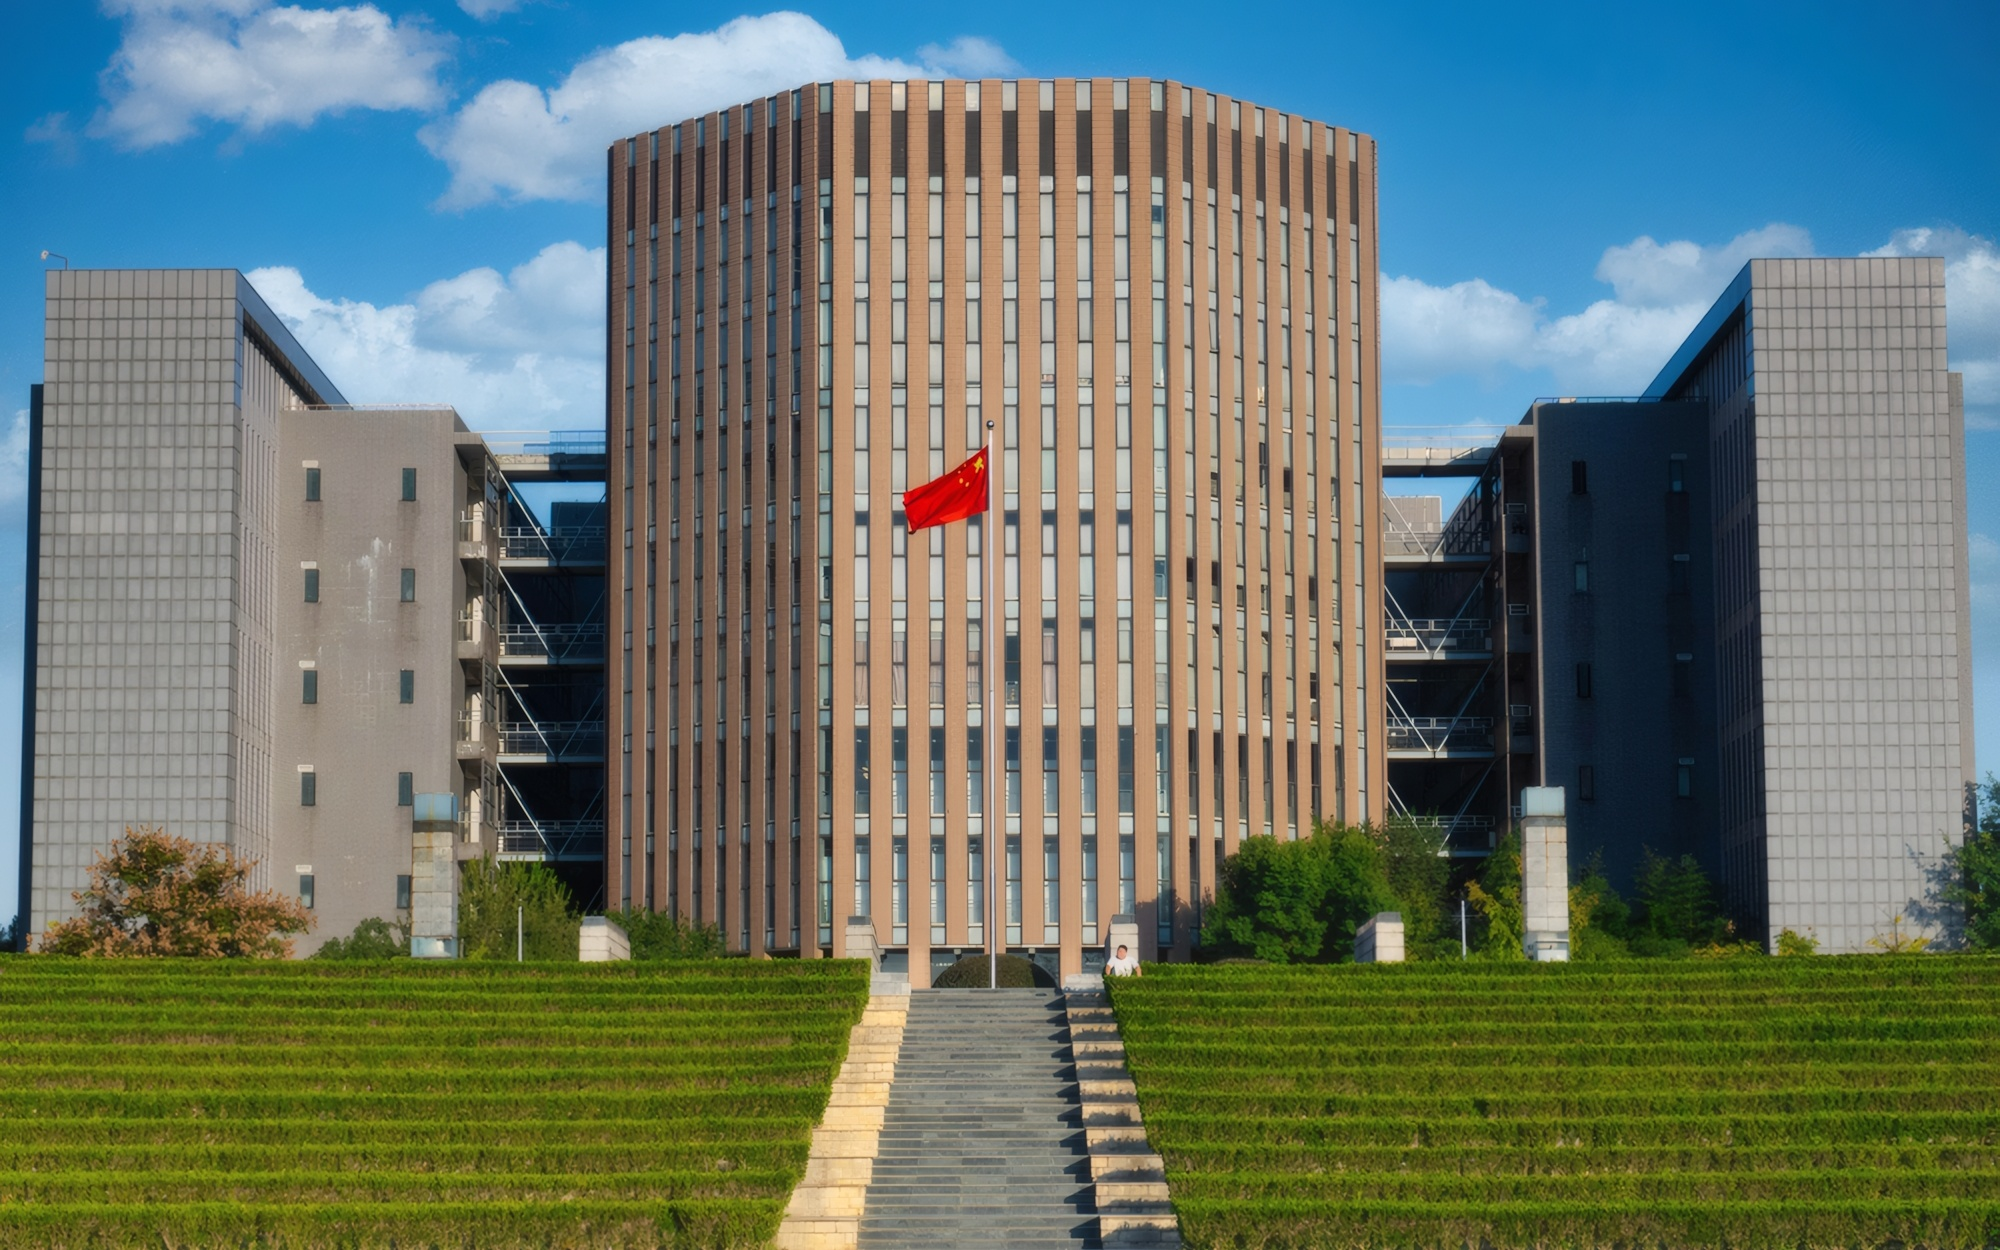
\includegraphics[width=0.85\linewidth]{src/example_ahu.jpg}

\vspace{0.5em}

\parbox[t]{\linewidth}{\centering
\structure{安徽大学}\\
磬苑校区校园一景}

\column{0.32\textwidth}
\centering
\footnotesize\begin{tabular}{@{}lcr@{}}
\toprule
\textbf{工具} & \textbf{版本} & \textbf{用途} \\
\midrule
XeLaTeX & 2024 & 编译 \\
biber   & 2.19 & 文献 \\
Make    & 4.4  & 构建 \\
\bottomrule
\end{tabular}

\vspace{0.5em}

\parbox[t]{\linewidth}{\centering
\structure{工具链}\\推荐配置}

\column{0.32\textwidth}
\centering
\begin{tikzpicture}[scale=0.6]
\draw[fill=yantex@main!20] (0,0) -- (1,1.5) -- (2,0) -- cycle;
\draw[fill=yantex@light] (0,0) rectangle (2,1.5);
\node at (1,0.75) {\Tiny AHU};
\end{tikzpicture}

\vspace{0.5em}

\parbox[t]{\linewidth}{\centering
\structure{TikZ绘图}\\简单几何图形}
\end{columns}
\end{frame}
